%-----------------------------------------------------------------------------
%-----------------------------------------------------------------------------
%  UNIVERSITY OF LIMERICK
%  MIT License
%  Copyright (c) 2025 Fatemeh Amerehi
%  Department of Computer Science (University of Limerick)

% The Dissertation Template for for Undergrad/Master/PhD Thesis
%------------------------------------------------------------------------------
% Adopted from the Dissertation Template for UW-Madison available at https://github.com/Lodour/wisc-thesis-template Copyright (c) 2024 Yue Gao MIT License
%
% 
%
% 
%
% Permission is hereby granted, free of charge, to any person obtaining a copy
% of this software and associated documentation files (the "Software"), to deal
% in the Software without restriction, including without limitation the rights
% to use, copy, modify, merge, publish, distribute, sublicense, and/or sell
% copies of the Software, and to permit persons to whom the Software is
% furnished to do so, subject to the following conditions:
%
% The above copyright notice and this permission notice shall be included in all
% copies or substantial portions of the Software.
%
% THE SOFTWARE IS PROVIDED "AS IS", WITHOUT WARRANTY OF ANY KIND, EXPRESS OR
% IMPLIED, INCLUDING BUT NOT LIMITED TO THE WARRANTIES OF MERCHANTABILITY,
% FITNESS FOR A PARTICULAR PURPOSE AND NONINFRINGEMENT. IN NO EVENT SHALL THE
% AUTHORS OR COPYRIGHT HOLDERS BE LIABLE FOR ANY CLAIM, DAMAGES OR OTHER
% LIABILITY, WHETHER IN AN ACTION OF CONTRACT, TORT OR OTHERWISE, ARISING FROM,
% OUT OF OR IN CONNECTION WITH THE SOFTWARE OR THE USE OR OTHER DEALINGS IN THE
% SOFTWARE.


%=============================================================================
% The dissertation should have double-spacing main text
%=============================================================================
% Notes:
%   - Use `\DoubleSpacing` because the `memoir` class ignores `setspace`
%   - See https://tex.stackexchange.com/questions/651036/
%=============================================================================

\documentclass[12pt,oneside,letterpaper, oldfontcommands]{memoir}

% Use this package
\usepackage{thesis}

% You can use any fonts, there is no formatting restriction.
\usepackage{lmodern}
\usepackage{tgpagella}
\usepackage{lipsum}
% Make cross references clickable, enable `hidelinks` to remove boxes
\usepackage[hidelinks]{hyperref}




% Set natbib style, you can use any packages you like
\usepackage{natbib}
\setcitestyle{authoryear,round}


%\setcitestyle{sort,compress,numbers,square,comma}

% These packages are for the sample document only
\usepackage{graphicx}
\usepackage{lipsum}
\usepackage{booktabs}
\usepackage[dvipsnames, table]{xcolor}
\usepackage{subcaption} 
\usepackage{caption}
\usepackage{tikz}
\tikzstyle{bag} = [align=center]
\usetikzlibrary{positioning, quotes, arrows.meta, decorations.pathmorphing}
\usepackage{setspace}
\usepackage{multirow}

\usepackage{amssymb, amsmath, amsfonts}

\newcommand{\tiniest}{\fontsize{4.7pt}{4.8pt}\selectfont}




\definecolor{darkblue}{HTML}{000052}

\hypersetup{
    colorlinks=true,
    citecolor=MidnightBlue, 
    linkcolor=RoyalBlue,
    urlcolor=PineGreen
}








% Define thesis information
\title{  \Large Your Dissertation Title: A Contribution to Knowledge at the University of Limerick \\[1.5cm]
\includegraphics[width=7.1cm]{photos/logonew2020.jpg} }


\author{Student Name}
\department{
The Name of Your Lab or Research Center Here\\
The Name of Your Department Here}
%

\deposityear{YYYY}
\defensedate{DD/MM/YYYY}

% Define committee members
\committeemember{ \small\textbf{Advisor:} Faculty Name, Department, University of Limerick}
\committeemember{\small\textbf{Advisor:} Faculty Name, Department, University }
\committeemember{\small\textbf{Examiner:} Faculty Name, Department, University}
\committeemember{\small\textbf{Examiner:} Faculty Name, Department, University }
\committeemember{\small\textbf{Chair:} Faculty Name, Department, University}



\dedication{
\begingroup
\color{MidnightBlue}  % Set text color
\begin{center}  % Maintain line breaks and spaces

Your Dedications Go Here \\
\lipsum[1][1]


\end{center}
\endgroup
}




\acknowledgements{

Your Acknowledgements Go Here \\
\lipsum[1]
}

\declaration{I herewith declare that I have produced this paper without the prohibited assistance of third parties and without making use of aids other than those specified; notions taken over directly or indirectly from other sources have been identified as such. This paper has not previously been presented in identical or similar form to any other Irish or foreign examination board. The thesis work was conducted from Year YYYY to YYYY under the supervision of Prof./Dr. Name at University of Limerick.

\vspace{10mm}
\noindent
Limerick, YYYY}




\abstract{
The abstract should provide a brief summary of your research, including the problem, methodology, results, and conclusion.

\lipsum[1]

}





% Set the depth of section numbers you like
\setcounter{secnumdepth}{3}

% Set the depth of table of contents you like
\setcounter{tocdepth}{3}




\begin{document}



% Generate title and preliminary pages
\maketitle
\makefrontmatter

% chapters


\chapter{Introduction}

The introduction serves to set the stage for your research and helps the reader understand the context and significance of your work. The following sections should be included in the introduction:


\begin{itemize}
    \item \textbf{Background and Context}: Provide an overview of the broad area your research is situated in. This is where you set the context for your work and explain why this area of study is important.
    
    \item \textbf{Research Problem}: Clearly define the specific research problem your thesis addresses. Describe the gap in existing knowledge that you aim to fill with your research.
    
    \item \textbf{Objectives and Research Questions}: State the specific objectives of your research. These are often framed as research questions or hypotheses you intend to explore throughout the thesis.
    
    \item \textbf{Methodology Overview}: Provide a brief summary of your research methods. This section should give an overview of the approach you used to gather data or conduct experiments, and how these methods align with the research objectives.
    
    \item \textbf{Significance of the Study}: Explain why your research matters. Discuss the potential contributions to the field, its relevance, and any practical applications of your findings.
    
    \item \textbf{Thesis Structure}: Outline the structure of your thesis. Briefly summarize the content of each chapter so the reader knows what to expect.
\end{itemize}



\lipsum[2-7]
\chapter{LaTeX Tutorial}

This section provides a brief tutorial on how to use LaTeX to insert links, write mathematical equations, and include figures in your thesis. These are some of the essential skills for formatting your document effectively.

\section{Inserting Links}
To insert a hyperlink in your LaTeX document, use the \texttt{hyperref} package. This package allows you to add clickable links to URLs, references, and even email addresses. Here’s how you can use it:

\begin{itemize}
    \item \textbf{Inline Math Mode}: For short formulas within text, enclose the math expression with dollar signs:
    \begin{verbatim}
    This is an inline equation:
    $ x = \frac{-b \pm \sqrt{b^2 - 4ac}}{2a}$.
    \end{verbatim} 
    which renders as \( x = \frac{-b \pm \sqrt{b^2 - 4ac}}{2a} \).

    \item \textbf{Displayed Math Mode}: For larger equations or equations that need to be centered on their own line, you can use the `equation` environment.

    \begin{verbatim}
    \begin{equation}
        x = \frac{-b \pm \sqrt{b^2 - 4ac}}{2a}
    \end{equation}
    \end{verbatim}

    This will display the equation on its own line and automatically number it, like this:
    \begin{equation}
    x = \frac{-b \pm \sqrt{b^2 - 4ac}}{2a}
    \end{equation}
    
    \item \textbf{Multiple Equations with Alignment}: To display multiple equations and align them at specific points, such as the equals sign, you can use the `align` environment, which requires the `amsmath` package.
    
    First, add the following to your preamble:
    \begin{verbatim}
    \usepackage{amsmath}
    \end{verbatim}
    
    Then, use the `align` environment:
    \begin{verbatim}
    \begin{align}
        x &= \frac{-b + \sqrt{b^2 - 4ac}}{2a} \\
        x &= \frac{-b - \sqrt{b^2 - 4ac}}{2a}
    \end{align}
    \end{verbatim}

    This will display two equations aligned at the equals sign, like this:
    \[
    x = \frac{-b + \sqrt{b^2 - 4ac}}{2a}
    \]
    and
    \[
    x = \frac{-b - \sqrt{b^2 - 4ac}}{2a}
    \]
    
    The `align` environment allows you to align multiple equations and gives each equation its own number.
\end{itemize}




\section{Tables with \texttt{natbib}}
The \texttt{natbib} package is commonly used for citation management in LaTeX, but it does not directly relate to tables. However, you can use it to cite sources in table captions.

To include the \texttt{natbib} package in your document, add the following in the preamble:

\begin{verbatim}
\usepackage{natbib}
\bibliographystyle{plainnat} % Or another style like abbrvnat
\end{verbatim}

To create a table, use the \texttt{tabular} environment:

\begin{verbatim}
\begin{table}[h]
    \centering
    \begin{tabular}{|c|c|c|}
        \hline
        Column 1 & Column 2 & Column 3 \\
        \hline
        Data 1 & Data 2 & Data 3 \\
        Data 4 & Data 5 & Data 6 \\
        \hline
    \end{tabular}
    \caption{Example Table \citep{author2025book}}
    \label{tab:example}
\end{table}
\end{verbatim}

This will create a table with three columns, as follows:


\begin{table}[h]
    \centering
    \begin{tabular}{ccc}
        \hline
        Column 1 & Column 2 & Column 3 \\
        \hline
        Data 1 & Data 2 & Data 3 \\
        Data 4 & Data 5 & Data 6 \\
        \hline
    \end{tabular}
    \caption{Example Table \citep{author2025book}}
    \label{tab:example}
\end{table}

% with citations in the caption. The \texttt{\citep} command from \texttt{natbib} allows in-text citations in the caption.


\section{Adding Pictures}
To include images, use the \texttt{graphicx} package:

\begin{verbatim}
\usepackage{graphicx}
\end{verbatim}

Example:

\begin{verbatim}
\begin{figure}[h]
    \centering
    \includegraphics[width=0.5\textwidth]{assets/images.png}
    \caption{The emblem of the University of Limerick.}
    \label{fig:image}
\end{figure}
\end{verbatim}



\begin{figure}[h]
    \centering
    \includegraphics[width=0.5\textwidth]{assets/images.png}
    \caption{The emblem of the University of Limerick.}
    \label{fig:image}
\end{figure}


To reference this image use \texttt{ref} as follows:


\begin{verbatim}
As shown in Figure \ref{fig:image}, the example...
\end{verbatim}




\section{Drawing with \texttt{TikZ}}

The \texttt{TikZ} package allows for drawing detailed scientific diagrams such as spacetime graphs. To use it, include the package  \texttt{tikz} in the preamble.

You can create various shapes and diagrams using LaTeX. For example, here is a spacetime diagram with vertical worldlines, light signals, and annotations. To find more information on how to create a similar diagram, visit \href{https://tikz.net/relativity_minkowski_diagram/}{this link}.

\begin{verbatim}
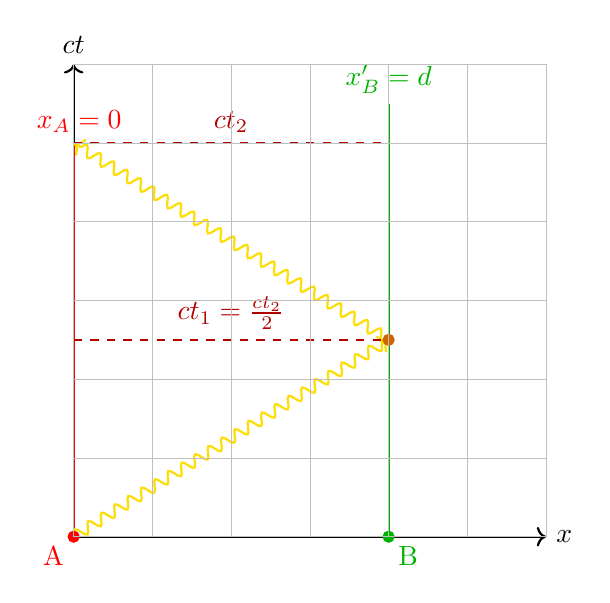
\begin{tikzpicture}
    % Axis
    \draw[->, thick] (0,0) -- (0,6) node[above] {\(ct\)};
    \draw[->, thick] (0,0) -- (6,0) node[right] {\(x\)};
    
    % Worldlines
    \draw[thick, red] (0,0) -- (0,5) node[above, xshift=2pt] 
    {\textcolor{red}{\(x_A = 0\)}};
    \draw[thick, green!70!black] (4,0) -- (4,5.5) node[above] 
    {\textcolor{green!70!black}{\(x'_B = d\)}};
    
    % Light paths
    \draw[->, thick, yellow!80!orange, 
    decorate, decoration={snake, amplitude=0.7mm, segment length=2mm}]
        (0,0) -- (4,2.5);
    \draw[->, thick, yellow!80!orange, 
    decorate, decoration={snake, amplitude=0.7mm, segment length=2mm}]
        (4,2.5) -- (0,5);

    % Dotted lines
    \draw[dashed, thick, red!70!black] 
    (0,2.5) -- (4,2.5) node[midway, above] 
    {\(ct_1 = \frac{ct_2}{2}\)};
    \draw[dashed, thick, red!70!black] 
    (0,5) -- (4,5) node[midway, above] {\(ct_2\)};
    
    % Events
    \filldraw[red] (0,0) circle (2pt) node[below left] {A};
    \filldraw[green!70!black] (4,0) circle (2pt) node[below right] {B};
    \filldraw[orange!80!black] (4,2.5) circle (2pt);

    % Grid (optional)
    \draw[step=1cm, lightgray, very thin] (0,0) grid (6,6);
\end{tikzpicture}
\end{verbatim}

This renders the following diagram:

\begin{figure}[h]
\centering
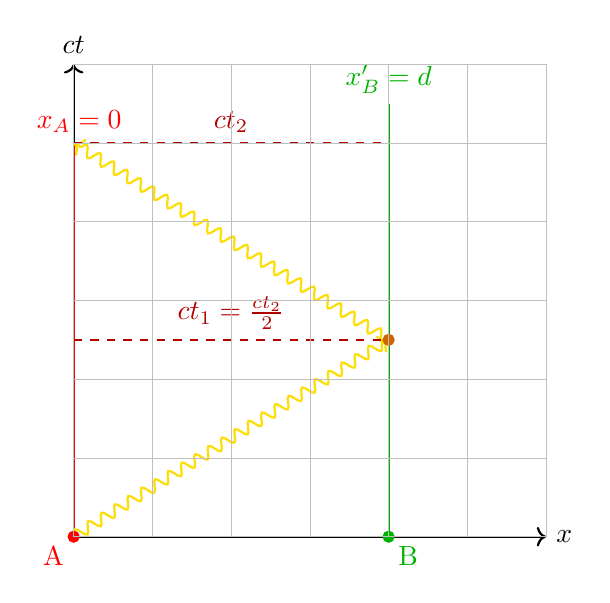
\begin{tikzpicture}
    % Axis
    \draw[->, thick] (0,0) -- (0,6) node[above] {\(ct\)};
    \draw[->, thick] (0,0) -- (6,0) node[right] {\(x\)};
    
    % Worldlines
    \draw[thick, red] (0,0) -- (0,5) node[above, xshift=2pt] {\textcolor{red}{\(x_A = 0\)}};
    \draw[thick, green!70!black] (4,0) -- (4,5.5) node[above] {\textcolor{green!70!black}{\(x'_B = d\)}};
    
    % Light paths
    \draw[->, thick, yellow!80!orange, decorate, decoration={snake, amplitude=0.7mm, segment length=2mm}]
        (0,0) -- (4,2.5);
    \draw[->, thick, yellow!80!orange, decorate, decoration={snake, amplitude=0.7mm, segment length=2mm}]
        (4,2.5) -- (0,5);

    % Dotted lines
    \draw[dashed, thick, red!70!black] (0,2.5) -- (4,2.5) node[midway, above] {\(ct_1 = \frac{ct_2}{2}\)};
    \draw[dashed, thick, red!70!black] (0,5) -- (4,5) node[midway, above] {\(ct_2\)};
    
    % Events
    \filldraw[red] (0,0) circle (2pt) node[below left] {A};
    \filldraw[green!70!black] (4,0) circle (2pt) node[below right] {B};
    \filldraw[orange!80!black] (4,2.5) circle (2pt);

    % Grid (optional)
    \draw[step=1cm, lightgray, very thin] (0,0) grid (6,6);
\end{tikzpicture}
\caption{Spacetime diagram showing light signal exchange between two observers.}
\label{fig:spacetimetikz}
\end{figure}

\newpage
\section{Using Citations}
To cite sources, use the \texttt{biblatex} package:

\begin{verbatim}
\usepackage{biblatex}
\addbibresource{references.bib}
\end{verbatim}

\subsection{Inline Citation Example}
Use \texttt{\textbackslash cite} to refer to an author within the text:

\begin{verbatim}
According to \cite{author2025book}, books are important.
\end{verbatim}

\subsection{Parenthetical Citation Example}
Use \texttt{\textbackslash parencite} to place citations in parentheses:

\begin{verbatim}
Books are an important source of knowledge \parencite{author2025book}.
\end{verbatim}

To list all references, add:

\begin{verbatim}
\printbibliography
\end{verbatim}

\textcolor{blue}{This is an example of using color in your document~\cite{author2024article,author2023conference}.}

\input{04_conclusion}

% The reference can use 1.5 spacing
\OnehalfSpacing

% Use any bib style you like
%bibliographystyle{agsm} %---> this is used in previous template but gives full authors sometimes rather than et.al.
\bibliographystyle{abbrvnat}


\bibliography{refrences.bib}

\end{document}


